\section{Formatting}
Sometimes we need as special symbols that are not available in keyboard. Then go \href{https://www.tutorialspoint.com/online_latex_editor.php}{{\color{blue}here}}, click that symbol you need and copy the command from text editor of {\color{red}Tutorials Point}.

\section{Font}
\subsection{Font Size}
Here the picture guide of Font-Size That we can use in "basicstyle" parameter at "lstset".
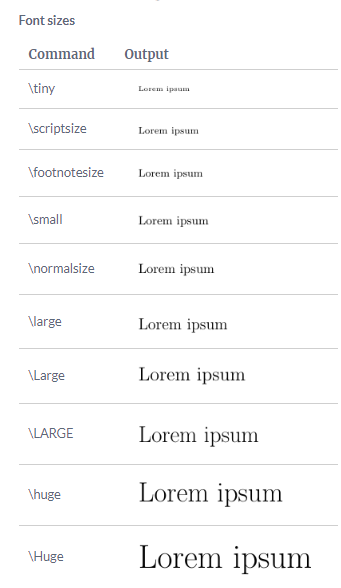
\includegraphics[scale=1]{../Font size.png}
\subsection{Font Face}

\section{Code Listing parameters}
Code listing parameters/options:\\
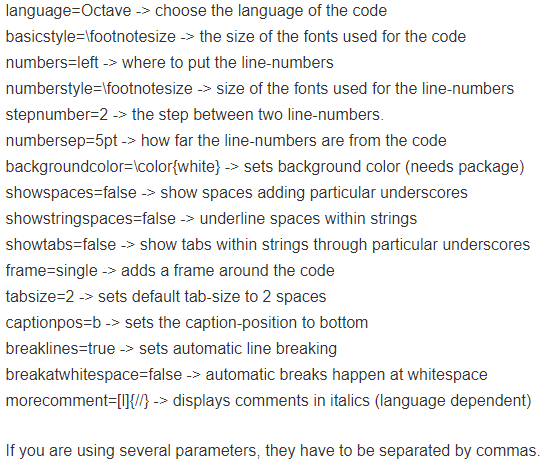
\includegraphics[width=290pt, height=300pt]{../Code listing parameters.png} 

\section{Shadow frame in code listing}
Picture guide of shadow fraem in listing:\\
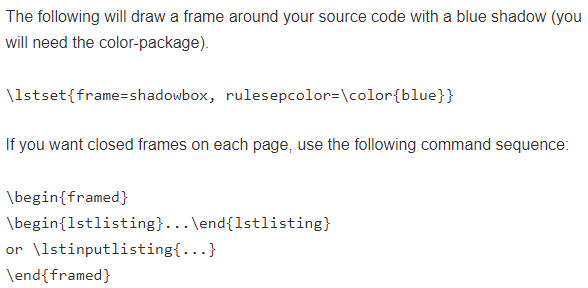
\includegraphics[scale=1]{../Shadow frame in code listing.png}

\section{Themes we can use in BEAMER class}
\subsection{Presentation themes without navigation bar}
\begin{enumerate}
 \item default
 \item boxes
 \item Bergen
 \item Boadilla
 \item Madrid
 \item AnnArbor
 \item CambridgeUS
 \item EastLansing
 \item Pittsburgh
 \item height=1 cm, Rochester
\end{enumerate}

\subsection{Presentation theme with a tree-like navigation bar}
\columnseprule = 0 mm
\begin{enumerate}
\begin{multicols}{2}
 \item Antibes
 \item JuanLesPins
 \item Montpellier
 \item Berkeley
 \item Goettingen
 \item Marburg
 \item Hannover
 \item Berlin
 \item Ilmenau
 \item Dresden
 \item Darmstadt
 \item Frankfurt
 \item Singapore
 \item Szeged
\end{multicols}
\end{enumerate}

\section{\href{https://www.overleaf.com/learn/latex/List_of_Greek_letters_and_math_symbols}{List of Greek letters and math symbols}}
There is a package documentation called Symbols.pdf and another package is fontawesome that provides icons of fontawesome.
\begin{center}
	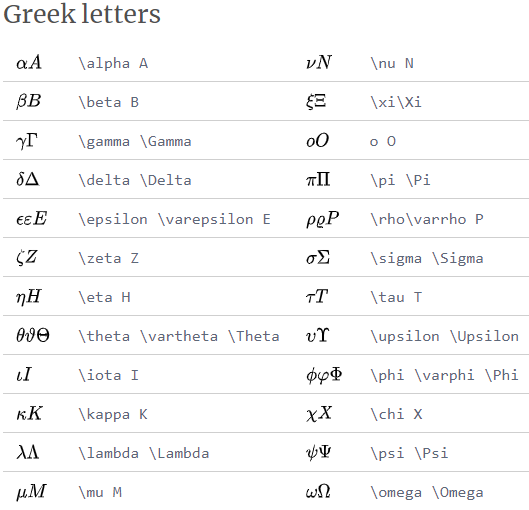
\includegraphics[width=200pt]{Source Images/Greek Letters.png}
	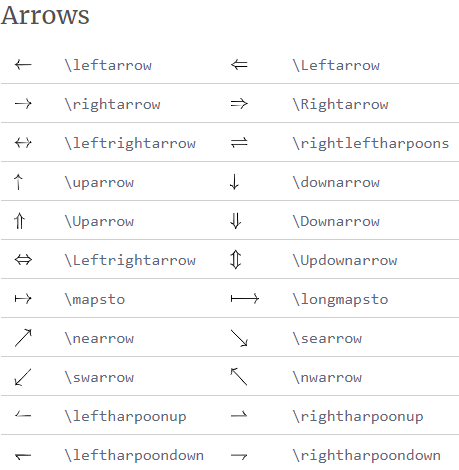
\includegraphics[width=200pt]{Source Images/Arrows.png}
	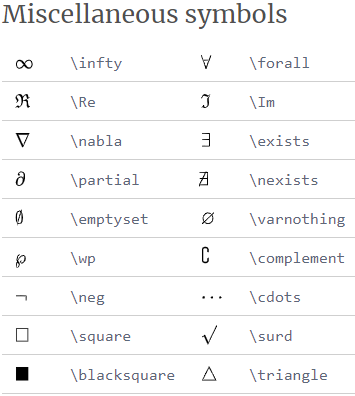
\includegraphics[width=200pt]{Source Images/Miscellaneous symbols.png}
	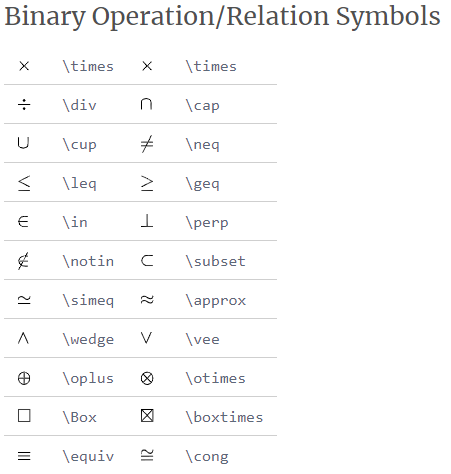
\includegraphics[width=200pt]{Source Images/Binary Operation-Relation Symbols.png}
\end{center}

\section{Available Document Structure Commands}
\subsection{BOOK and REPORT}
\begin{itemize}
	\item part
	\item chapter
	\item section
	\item subsection
	\item subsubsection
	\item paragraph
	\item subparagraph
\end{itemize}

\subsection{ARTICLE}
\begin{itemize}
	\item part
	\item section
	\item subsection
	\item subsubsection
	\item paragraph
	\item subparagraph
\end{itemize}

\section{XeLaTeX}
\textcolor{blue}{XeLaTeX} is replacement for PDFLaTeX, it will takes input form LaTeX and turns output into a PDF. You cannot see instant created PDF file besides of TeXMaker.\linebreak
The major differences between \LaTeX{}/PDF\LaTeX{} are:

\begin{itemize}
	\item \textcolor{blue}{XeLaTeX} assumes input is in UTF-8(which allows encoding of non-English and non-Latin characters) by default.
	\item \textcolor{blue}{XeLaTeX} uses system fonts, not specially installed \LaTeX{} fonts.
\end{itemize}

It's packaged with TeXLive distribution of \LaTeX{}.

\section{The "hyperref" Package}
Include as \texttt{\textbackslash usepackage[hidelinks]{hyperref}} For adding hyperlink / clickable link. \textit{hidelinks} will remove red frame form all type of links. While importing this package, it has to be the last package that are included. Because of, The \textit{hyperref} documentation says, "Make sure it comes last of your loaded packages". The reason is that it redefines many \LaTeX{} commands. It's a rule of thumb that helps you to avoid error. Also that, the \textit{amsrefs} user guide notes that, this package has to become after \textit{hyperref}.

\section{Background Image}
There are many different ways to add a background image to a latex file/page.

\subsection{Package "background"}
For further details, see manual.pdf or download it from CTAN's official website. The package offers the placement of background material on the pages of a document. The user can control many aspects(contents, position, color, opacity) of the background material that will be displayed; all placement and attribute settings are controlled by setting key values.

\section{Default Font Face used in \LaTeX{}}
\textbf{Computer Modern} is the original family of typefaces used by the typesetting program TeX. It was created by \textbf{Donald Knuth} with his Metafont program and was most recently updated in 1992. It widely used in scientific publishing, especially in disciplines that make frequent use of mathematical notation. Category: Serif.